\documentclass{article}

\usepackage[a4paper, total={7in, 10in}]{geometry}
\usepackage[utf8]{inputenc}

\usepackage{amsmath}
\usepackage{enumitem}
\usepackage{float}
\usepackage{graphicx}
\usepackage{hyperref}
\usepackage{multicol}
\usepackage{stmaryrd}
\usepackage{subcaption}

\title{MPRI 2-24-2 Homework Project}
\author{Rémi Dupré, Garance Gourdel}
\date{February 2019}


% Bullet points configuration
\setlist{noitemsep}


\begin{document}

\maketitle

\section{Introduction: LABS}

  The problem is defined in \cite{Packebusch_2016} as the following: consider a
  sequence $S = (s_1, ..., s_N)$ with $s_i = \pm 1$. The autocorrelations of S
  are defined as follow:
    $$C_k(S) = \sum\limits_{i=1}^{N-k} s_i s_{i+k}$$

  For $k = 0, 1, ..., N-1$ and the ``energy'' of S is defined as the sum of the
  squares of all off-peak correlations
    $$E(S) = \sum\limits_{k=1}^{N-1} C_k^2(S)$$

  The \textit{low-autocorrelation binary sequence} (LABS) problem is to find a
  sequence S of given length $N$ that minimizes $E(S)$ or, equivalently,
  maximizes the \textit{merit factor}
    $$F(S) = \frac{N^2}{2 E(S)}$$

  This maximization problem has applications in communications engineering (as
  it is used to find modulation pulses in radar and sonar ranging) and physics
  (where $E(S)/N$ can be interpreted as the energy of $N$ interacting Ising
  spins).

  As for the state of the art on the problem, we already mentioned
  \cite{Packebusch_2016} from Tom Packebusch and Stephan Mertens, the paper
  from Borko Bošković, Franc Brglez, Janez Brest
  \cite{DBLP:journals/asc/BoskovicBB17} is also a good complement.


\section{Implemented Algorithm}

  All our tests are developed using C++ 14, compiled with gcc 8.2.1 and the
  \textit{-O3} and \textit{-Ofast} flags. The plots are automatically generated
  through Python (matplotlib), our code is available on GitHub :
  \href{https://github.com/remi-dupre/LABS}{https://github.com/remi-dupre/LABS}.

  Our code is structured as follow: all our optimizers inherit from a generic
  class \texttt{Optimizer} that holds a seed and the size of the search space.
  Theses optimizers implement a method \texttt{run} which takes an object of
  type \texttt{LabsInstance} as input. This type \texttt{LabsInstance} is used
  to interact with the problem in a blackbox or near-blackbox way while
  tracking merit of current evaluated sequences and runtime of the algorithm:

  \begin{itemize}
    \item It can evaluate the merit of a given sequence in a blackbox way with
      complexity $O(N^2)$.
    \item It can enter a ``local mode'' during which it can only swap one spin
      at once but with complexity $O(N)$. Entering this local mode costs time
      $O(N^2)$, of course, an algorithm using this mode can't properly be
      considered as a blackbox approach.
  \end{itemize}

  We didn't implement any way to bound the running time of an algorithm, thus
  our algorithms are free to run for an arbitrary duration, usually related to
  a given \texttt{iterations} parameter.

  In the following subsections, we describe the different algorithms we
  implemented, attached with a chart showing the evolution of the merit of the
  sequences the algorithm evaluates over time with $N = 300$. The dark blue
  line represent the evolution of the best merit reached at a step of the
  algorithm and the lighter blue represents arbitrary evaluations done by the
  algorithm. Usually we represent all evaluation done by the algorithm but for
  simulated annealing we represent only the evaluation that where saved, those
  who were bad but not more than the defined threshold.


\subsection{Full Random}

  This algorithm is as simple as it can be, it keeps the best sequence out of a
  given number of independently uniformly picked sequences. It is obviously
  quite inefficient but it was mainly implemented to test our initial code and
  get an idea of the order of magnitude of a result for a bad algorithm.

  \begin{multicols}{2}

    \subsubsection*{Parameters of the algorithm}
      \begin{itemize}
        \item \texttt{seq\_size} ($N$): size of search space
        \item \texttt{iterations}: number of selected sequences
      \end{itemize}

    \subsubsection*{Typical orders of magnitude ($N = 300$)}

      \begin{itemize}
        \item \texttt{iterations}: $10,000$
        \item running time: $0.55s$
        \item merit: $1.60$
      \end{itemize}

    \vphantom{0}

  \columnbreak

    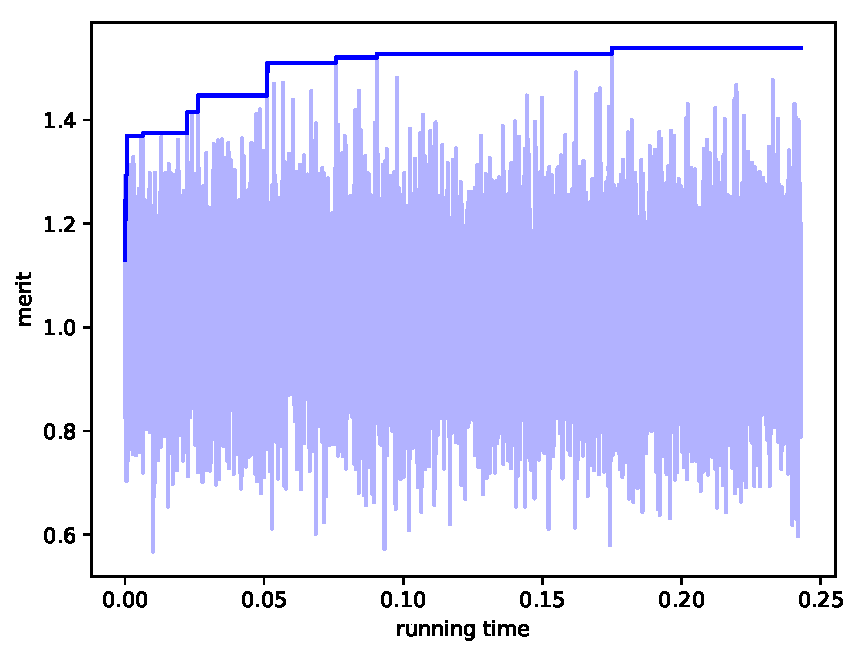
\includegraphics[width=\linewidth]{figures/convergence_full_random.pdf}

  \end{multicols}


\subsection{Local Search}

  This algorithm is very close to the previous one, but it doesn't restrict
  itself to a blackbox setting. Instead of picking up independently sequences,
  each iteration of this algorithm only swaps one spin of last evaluated
  sequence. After $O(N)$ swaps (and thus $O(N^2)$ steps), the sequence is
  likely to be equivalent to a sequence picked from an uniform distribution.

  \begin{multicols}{2}

    \subsubsection*{Parameters of the algorithm}
      \begin{itemize}
        \item \texttt{seq\_size} ($N$): size of search space
        \item \texttt{iterations}: number of spin swaps
      \end{itemize}

    \subsubsection*{Typical orders of magnitude ($N = 300$)}

      \begin{itemize}
        \item \texttt{iterations}: $1,000,000$
        \item running time: $0.55s$
        \item merit: $1.85$
      \end{itemize}

    \vphantom{0}

  \columnbreak

    \includegraphics[width=\linewidth]{figures/convergence_local_search_simple.pdf}

  \end{multicols}

\subsection{Local Search With Maxima Seeking}

  This incorporates an extra step after each iteration of the local search.
  While the algorithm didn't reach a local maximum (where swapping any spin
  would decrease the merit), it choose uniformly a bit to swap that increases
  the merit of the sequence. Notice that this is quite close to a simulated
  annealing algorithm.

  \pagebreak
  \begin{multicols}{2}

    \subsubsection*{Parameters of the algorithm}
      \begin{itemize}
        \item \texttt{seq\_size} ($N$): size of search space
        \item \texttt{iterations}: number of spin swaps
        \item \texttt{seek\_local\_maximum}: if set to 1, it means that the
          maxima seeking is activated, otherwise it performs a naïve local
          search.
      \end{itemize}

    \subsubsection*{Typical orders of magnitude ($N = 300$)}

      \begin{itemize}
        \item \texttt{iterations}: $1,000,000$
        \item running time: $0.66s$
        \item merit: $5.1$
      \end{itemize}

    \vphantom{0}

  \columnbreak

    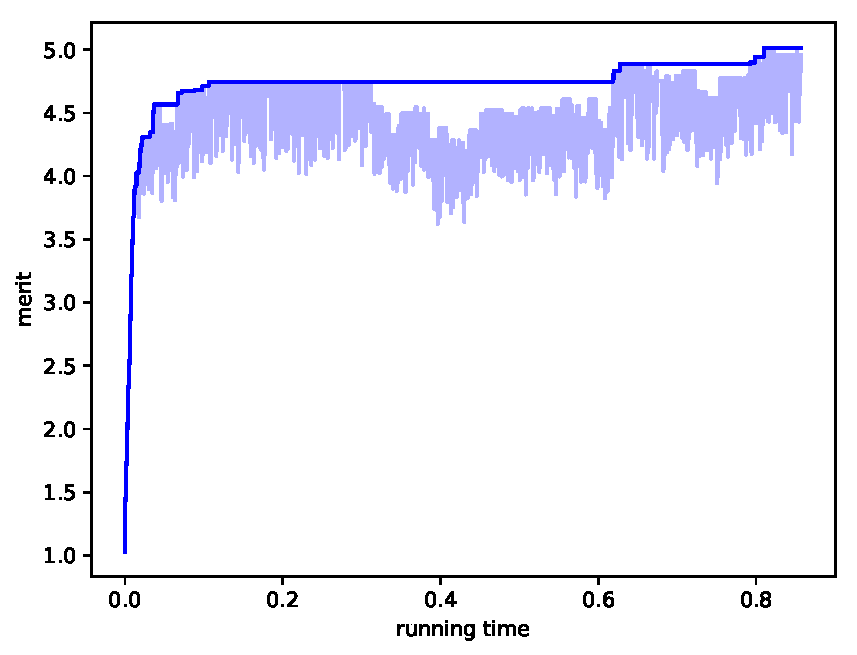
\includegraphics[width=\linewidth]{figures/convergence_local_search.pdf}

  \end{multicols}

\subsection{Threshold local search}

  Here, instead of searching mainly for the local minimas and then trying
  different thins as in the previous algorithm we blindly accept to swap a bit
  either if it improves the result of the algorithm or if it decreases by less
  than a defined threshold. We do that for three quarter of the number of
  iterations and than for the quarter remaining we only accept the improving
  swaps, in other word from there we do a local search.

 \begin{multicols}{2}
    \subsubsection*{Parameters of the algorithm}

      \begin{itemize}
        \item \texttt{seq\_size} ($N$): size of search space
        \item \texttt{iterations}: theoretical number of iteration of the
          algorithm, not in used now
        \item \texttt{threshold}: the threshold to accept a "bad" swap
      \end{itemize}

    \subsubsection*{Typical orders of magnitude ($N = 300$)}

      \begin{itemize}
        \item \texttt{iterations}: $100000$
        \item \texttt{threshold}: $0.04$
        \item running time: $0.01s$
        \item merit: $4.33$
      \end{itemize}

    \vphantom{0}

  \columnbreak

    \includegraphics[width=\linewidth]{figures/convergence_threshold_localsearch.pdf}

  \end{multicols}

\subsection{Simulated annealing}

  There we keep the idea of accepting to not always maximize the merit but
  refine it to get a more 'scalable' solution that has a chance to give better
  result if we give it more time (which is not the case for threshold local
  search). Our implementation of the simulated algorithm was greatly helped by
  Mathieu Fehr and it is basically the same algorithm (reimplemented). Mathieu
  mainly based his work on \cite{KirkpatrickOptimizationBS}.

  In this algorithm, for every iteration:

  \begin{itemize}
    \item we swap a random bit
    \item we compute the new energy
    \item we accept the sequence if and only if $exp(\frac{old\_energy-
      new\_energy}{temperature})$ is greater than a random number between 0 and
      1.
    \item we decrease the temperature by multiplying it by $0.95$ every $2000$
      steps.
  \end{itemize}

  \pagebreak

  \begin{multicols}{2}

    \subsubsection*{Parameters of the algorithm}
      \begin{itemize}
        \item \texttt{seq\_size} ($N$): size of search space
        \item \texttt{iterations}: theoretical number of iteration of the
          algorithm, not in used now.
        \item \texttt{temperature}: the starting temperature that will moderate
          how soon we will start accepting worse merit.
      \end{itemize}

    \subsubsection*{Typical orders of magnitude ($N = 300$)}
      \begin{itemize}
        \item \texttt{iterations}: $500000$
        \item \texttt{temperature}: $1300$
        \item running time: $0.7s$
        \item merit: $4.88$
      \end{itemize}

    \vphantom{0}

  \columnbreak

    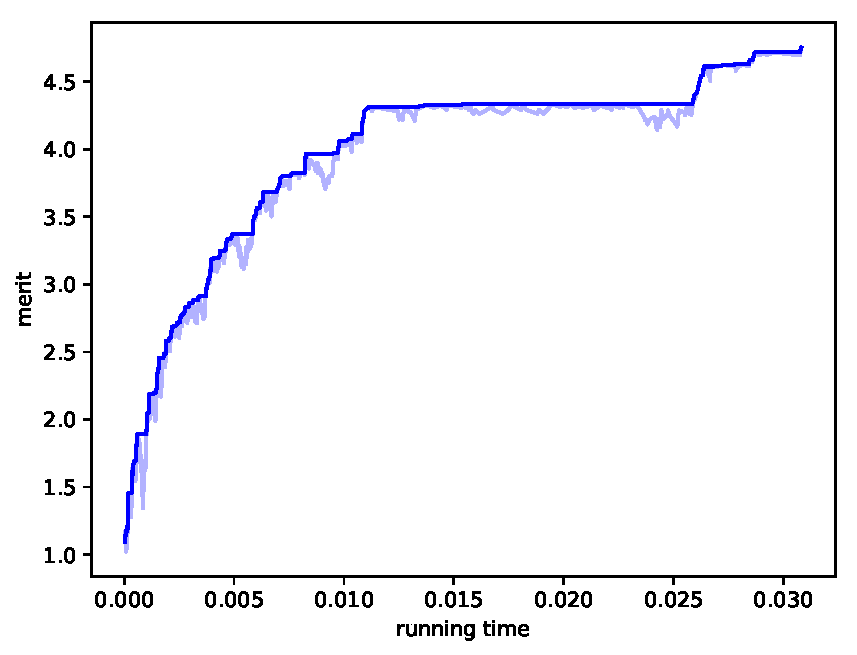
\includegraphics[width=\linewidth]{figures/convergence_simulated_annealing.pdf}

 \end{multicols}

\subsection{Genetic}

  This implementation of a genetic algorithm starts from a pool of
  \texttt{nb\_parents} random sequence. Starting from them we create
  \texttt{nb\_children} new sequences by taking, for each child, a pair of
  random parent and giving the child the bit value of the first parent or the
  second parent randomly (one chance over two). We then select the
  \texttt{nb\_parents} best children (those with the highest merit) and iterate
  the process until the algorithm stabilizes (i.e. we get the same best merit
  among the children 30 times).

  \begin{multicols}{2}
    \subsubsection*{Parameters of the algorithm}
      \begin{itemize}
        \item \texttt{seq\_size} ($N$): size of search space
        \item \texttt{iterations}: theoretical number of iteration of the
          algorithm, not in used now
        \item \texttt{nb\_parents}: number of parents
        \item \texttt{nb\_children}: number of children to generate from the
          parents
      \end{itemize}

    \subsubsection*{Typical orders of magnitude ($N = 300$)}
      \begin{itemize}
        \item \texttt{nb\_parents}: $100$
        \item \texttt{nb\_children}: $300$
        \item running time: $1.1s$
        \item merit: $3.0$
      \end{itemize}

    \vphantom{0}

  \columnbreak

    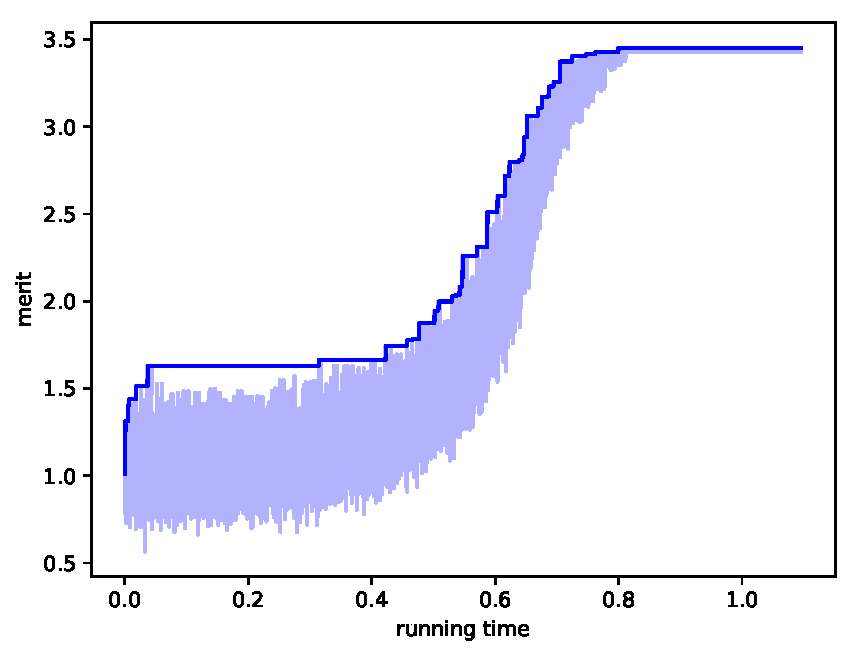
\includegraphics[width=\linewidth]{figures/convergence_genetic.pdf}

  \end{multicols}


\subsection{Maximize Correlation}

  At each iteration of this algorithm, it picks uniformly a $k \in \llbracket
  1, N-1 \rrbracket$ and swaps a spin $i$ such that $i$ is the choice of spin
  which results with the biggest $C_k$ after the operation.

  Given a sequence $S$ and a choice of autocorrelation $k$, a choice of the
  best spin to swap in order to increase $C_k$ can be done in O($N$) time by
  looking at $\Delta_i C_k$, where $\Delta_i C_k$ is the variation of $C_k$
  when swapping spin of index $i$ for the current sequence S:

    \[\forall i \in \llbracket 1, N \rrbracket,\  \Delta_i C_k =
      \begin{cases}
        -2 (s_i \times s_{i-k}) & \text{if } i > k \\
        \quad\quad\quad\quad  0 & \text{otherwise}
      \end{cases}
      +
      \begin{cases} 
        -2 (s_i \times s_{i+k}) & \text{if } i \leq N-k \\
        \quad\quad\quad\quad  0 & \text{otherwise}
      \end{cases}
   \]

  \pagebreak

  \begin{multicols}{2}
    \subsubsection*{Parameters of the algorithm}

      \begin{itemize}
        \item \texttt{seq\_size} ($N$): size of search space
        \item \texttt{iterations}: number of spin swaps
      \end{itemize}

    \subsubsection*{Typical orders of magnitude ($N = 300$)}

      \begin{itemize}
        \item \texttt{iterations}: $500$
        \item running time: $0.50s$
        \item merit: $3.6$
      \end{itemize}

    \vphantom{0}

  \columnbreak

    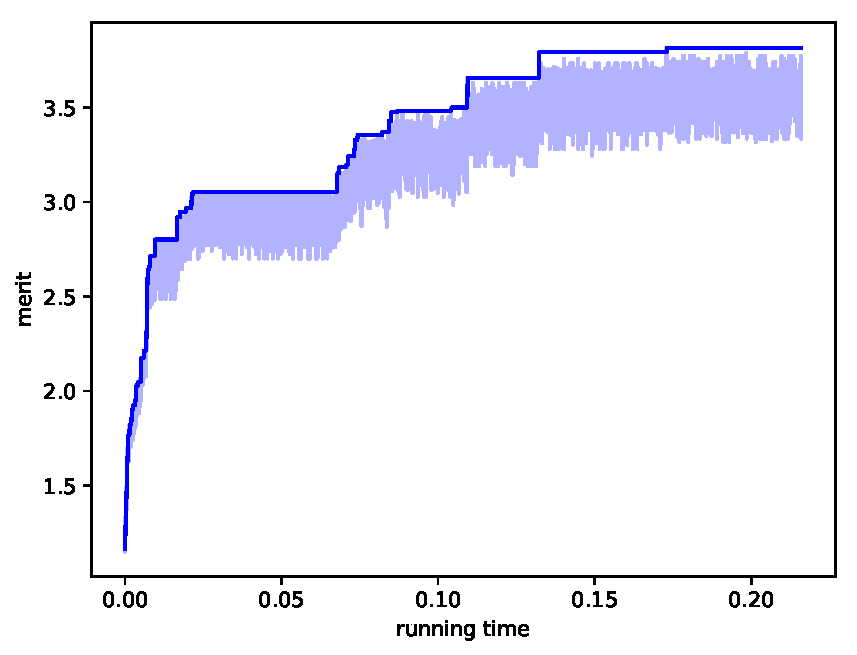
\includegraphics[width=\linewidth]{figures/convergence_maximize_correlation.pdf}

  \end{multicols}


\subsection{Harmonic Search}

  This algorithm came out of the idea that the definition of the problem seems
  to raise a concept of periodicity in the sequence. Swapping a chain of bits
  with indexed spaced by $k$ won't change the autocorrelation $C_k$ of the
  sequence.

  At each iteration, this algorithm uniformly picks a period $p$ and an offset
  $l$ and swaps the bits of index $p \cdot x + l$ and replace the sequence with
  the newly obtained one if it has a better merit. As it often pick a big
  period, it is helpful to swap the spins independently while computing the
  merit like in the local search algorithm.

  \begin{multicols}{2}
    \subsubsection*{Parameters of the algorithm}
      \begin{itemize}
        \item \texttt{seq\_size} ($N$): size of search space
        \item \texttt{iterations}: number of period swaps
      \end{itemize}

    \subsubsection*{Typical orders of magnitude ($N = 300$)}
      \begin{itemize}
        \item \texttt{iterations}: $50,000$
        \item running time: $0.33s$
        \item merit: $4.0$
      \end{itemize}

    \vphantom{0}
  \columnbreak
    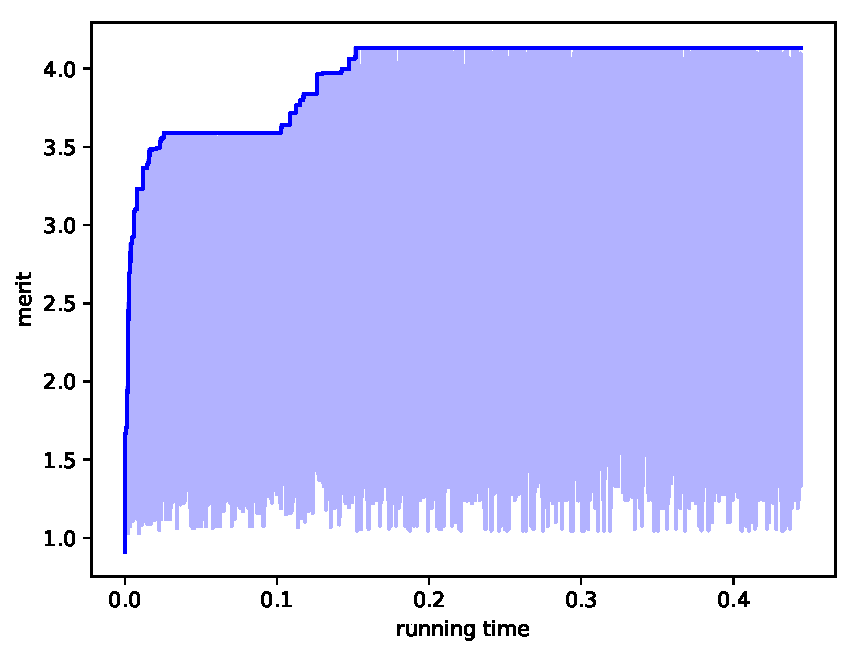
\includegraphics[width=\linewidth]{figures/convergence_harmonic_search.pdf}
  \end{multicols}


\subsection{Local Branching}

  This algorithm is a generalisation of how to seek a local minima. First, it
  computes a random ordering of the indexes. Then, for each index (in the
  obtained order), it swaps the bit of this index if it improves the merit.
  During this process, it is allowed to to make $k$ bad decisions (i.e.
  choosing to swap $k$ spins while decreasing the merit). The algorithm runs
  all bad decisions possibilities, sadly it is not possible to test this for a
  big $k$ value since it runs in $O(n^{2+k})$.

  \pagebreak
  \begin{multicols}{2}
    \subsubsection*{Parameters of the algorithm}
      \begin{itemize}
        \item \texttt{seq\_size} ($N$): size of search space
        \item \texttt{maximal\_depth} ($k$): maximal number of bad decisions
      \end{itemize}

    \subsubsection*{Typical orders of magnitude ($N = 300$)}
      \begin{itemize}
        \item \texttt{maximal\_depth}: $1$
        \item running time: $0.05s$
        \item merit: $3.1$
      \end{itemize}

    \vphantom{0}
  \columnbreak
    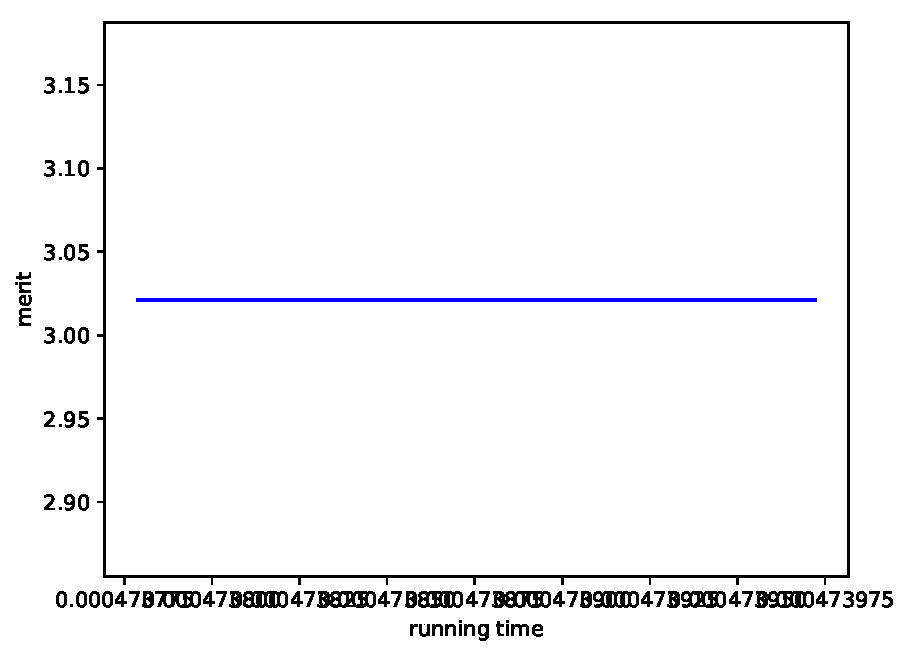
\includegraphics[width=\linewidth]{figures/convergence_local_branching.pdf}
  \end{multicols}


\section{Results}

  To compare the algorithms, we ran them all with the default parameters, each
  10 times to be able to extract a mean and a max over those ten execution. We
  did this over a range of different values for $N$ to get a global picture of
  the performance of the algorithms. We also measure the CPU time taken for each
  execution and the number of evaluation of the function, thus we can plot
  graph of the merit depending on the dimension, the runtime or number of
  evaluations depending on the dimension. We also have a system that allow for
  measure the merit or runtime depending on the different parameter of the
  heuristics.

  As we have implemented various algorithm to play with the problem and get a
  sense of what was working or not, analyzing them all in detail in this report
  would have been a tedious work (and we are already reaching the 5 pages
  limit). So we choose to detail the global comparison of our heuristic (each
  of them running at there best parameters chosen by some experimental
  sampling), and leave the evaluation of our parameters for some specific
  algorithm for the oral presentation.

    \begin{figure}[ht]
    \centering
    \scalebox{0.7}{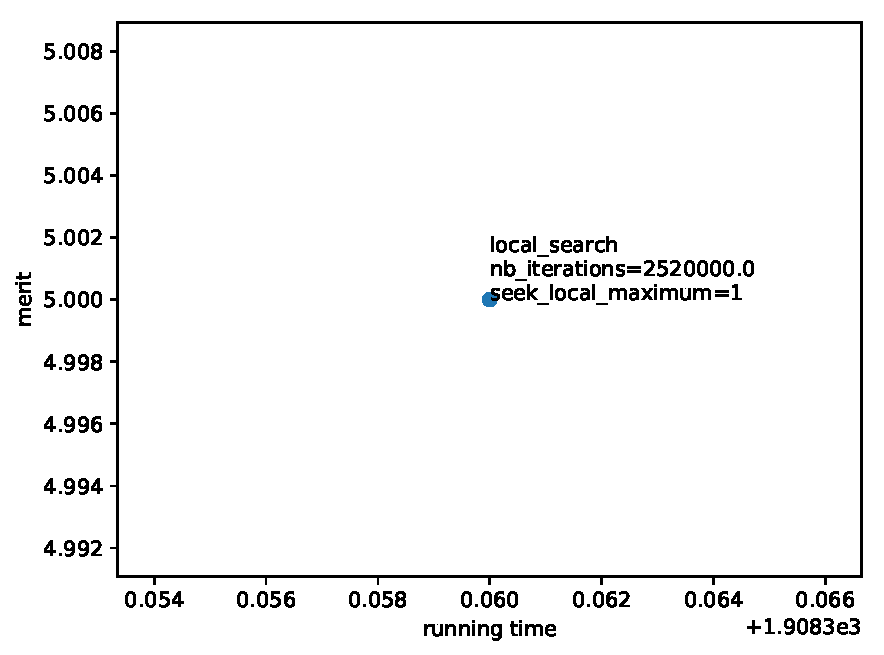
\includegraphics[]{figures/compare_300.pdf}}
    \caption{Comparison of results and running time of the different algorithms}
    \label{compare_points}
  \end{figure}

  When comparing the performances, what appears clearly on figure
  \ref{compare_points} is that the algorithms close to a simulated annealing
  (simulated\_annealing, threshold\_localsearch and local search with parameter
  seek\_local\_maximum enabled) are performing the best among algorithms we
  implemented, and it doesn't seem to depend of the dimension (cf. figure
  \ref{compare_merit}).

  \begin{figure}[H]
    \centering
    \begin{subfigure}[b]{0.49\textwidth}
      \centering
      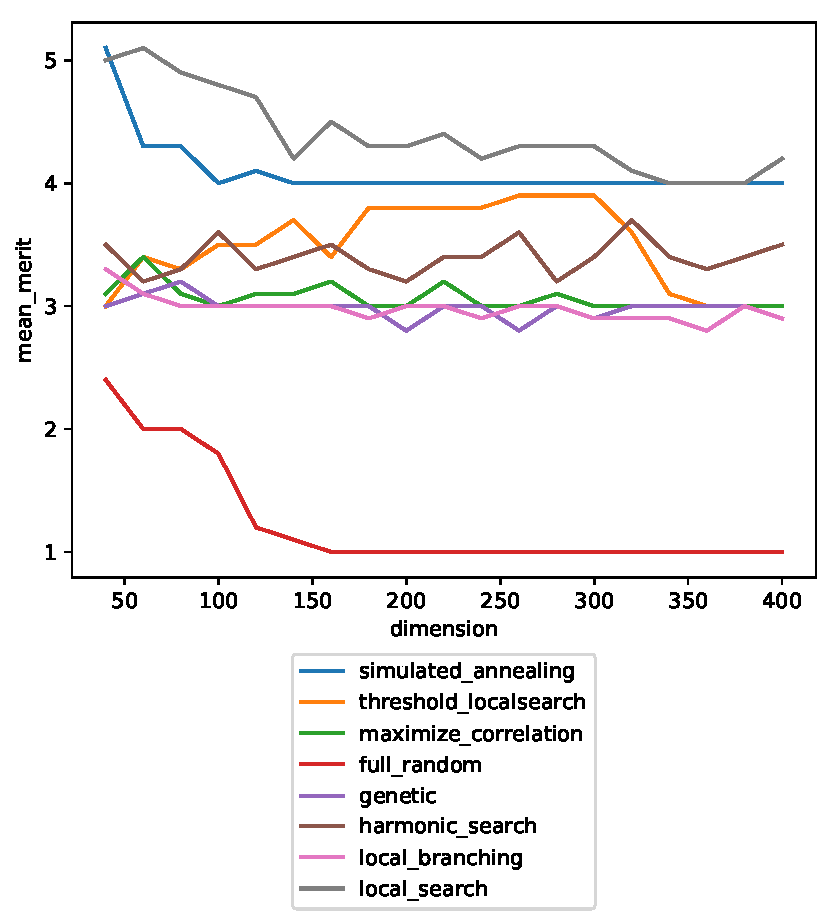
\includegraphics[width=\textwidth]{figures/dimension_mean_merit.pdf}
      \caption{Mean merit}
        \label{compare_merit_mean}
    \end{subfigure}
    \begin{subfigure}[b]{0.49\textwidth}
      \centering
      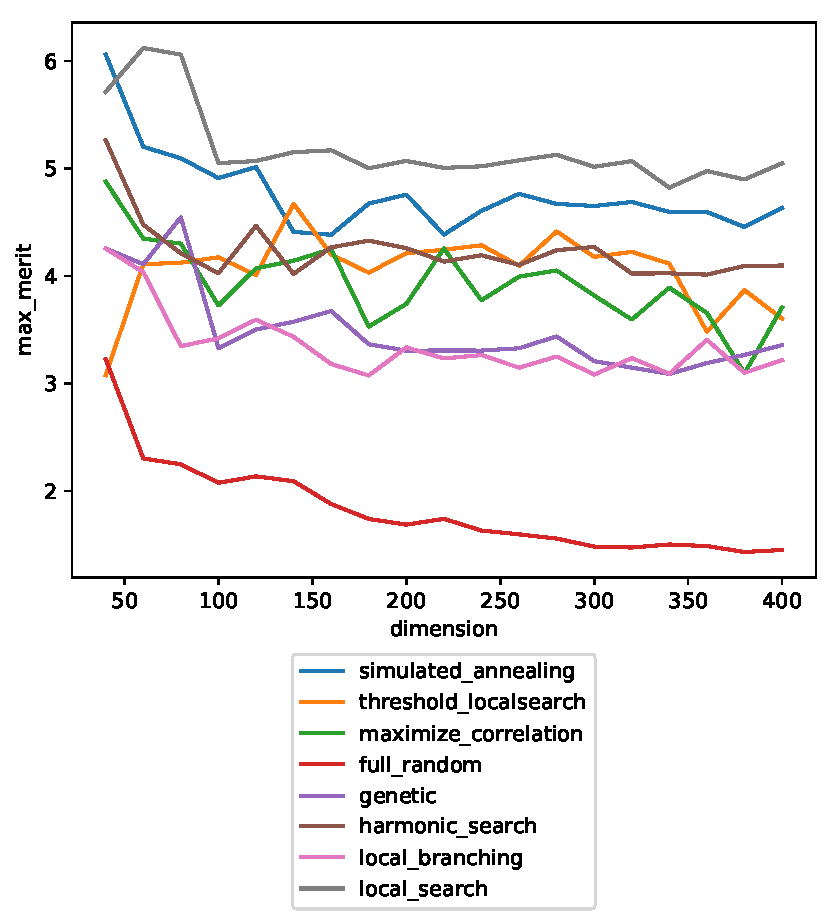
\includegraphics[width=\textwidth]{figures/dimension_max_merit.pdf}
      \caption{Max merit}
        \label{compare_merit_max}
    \end{subfigure}
    \caption{Performances of the algorithms over increasing dimensionality}
    \label{compare_merit}
  \end{figure}


  There appear to be a threshold on the difficulty of getting a better merit
  than 3 appearing on figure \ref{compare_merit_mean}, and our best algorithms
  hardly reach a value far better than 5.

  Our algorithm all have a complexity that is at least in $O(N^2)$, however it
  doesn't seem to appear, the running time of the algorithms appear to increase
  linearly when we increase the value of $N$ (figure \ref{compare_runtime}).

  \begin{figure}[H]
    \centering
    \begin{subfigure}[t]{0.35\textwidth}
      \vfil
      \centering
      \includegraphics[width=\textwidth]{figures/dimension_eval.pdf}
    \end{subfigure}
    \begin{subfigure}[t]{0.35\textwidth}
      \vfil
      \centering
      \includegraphics[width=\textwidth]{figures/zoom_dimension_eval.pdf}
    \end{subfigure}
    \begin{subfigure}[t]{0.35\textwidth}
      \centering
      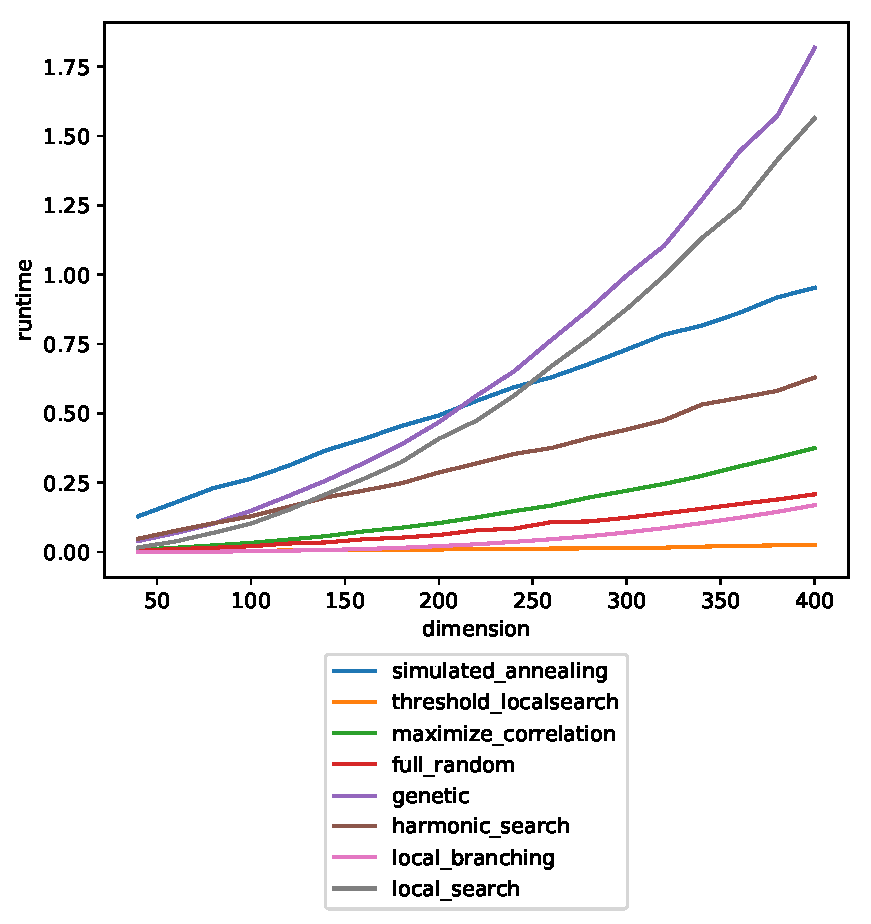
\includegraphics[width=\textwidth]{figures/dimension_runtime.pdf}
    \end{subfigure}
    \caption{Cost of the algorithms while increasing dimensionality}
    \label{compare_runtime}
  \end{figure}

  On figure \ref{compare_runtime} we show both our result in terms of
  evaluation of the merit and CPU runtime as for the heuristic that can run in
  'local mode' (described at the  beginning of the fist section), the cost of
  an evaluation is much cheaper ($O(N)$ instead of $O(N^2)$).

  As this is our best algorithm, we tested the local search with minima seeking
  algorithm with an higher iteration setting, allowing it to run each test for
  roughly 45 minutes. On its best run, its reached a merit value of $5.46$, but
  already seemed to stabilizes rather quickly.


\section{Conclusion}

  Despite the fact that our best result are all based on "accepting to pursue a
  sequence with a merit lower than the maximum we have seen so far", it was
  interesting to notice the difference of result based on the implementation of
  this philosophy. More precisely, it was interesting to see how a very simple
  heuristic like threshold-local-search could obtain a good solution very
  quickly.

  Some more original algorithms like the harmonic one could also be developed
  to get better results, however we didn't spend enough time to determine if
  they could be enhanced and as efficient as a simulated annealing.

\bibliography{labs}{}
\bibliographystyle{plain}

\end{document}

